In realen System kommt es immer zu Unsicherheiten oder Veränderungen welche das System- und Regelverhalten beeinflussen.
Die Methode der Polbereichsplatzierung, basierend auf dem  Multi-Modell-Ansatz, versucht die lineare Zustandsregelung von Systemen mit schwankenden oder unsicheren Parametern zu ermöglichen.
Die Erklärungen im nachfolgenden Abschnitt basieren auf den Ausführungen in \cite{RobReg} und \cite{Schaub}.

Zunächst wird das System in Abhängigkeit eines Parametervektors $\Theta$ wie folgt definiert
\begin{align}
	\dot{\w{x}} &= \M{A}(\Theta)\w{x} + \M{B}(\Theta)\w{u}\, , \qquad \w{x}(0) = \w{x}_0\\
	\w{y} 		&= \M{C}(\Theta)\w{x}
\end{align}
Das System besitzt die Ordnung $n$. Des Weiteren gilt $\w{u}\in\mathbb{R}^p$ und $\w{y}\in\mathbb{R}^q$. Es sind also $p$ Stellgrößen und $q$ Ausgangsgrößen vorhanden.
Der Parametervektor $\Theta$ beschreibt die veränderlichen Parameter des Systems. Beim Multi-Modell-Ansatz wird nun das System an $\Omega$ Stützstellen um $\Theta_{\rho}$ linearisiert. Somit erhält man eine Menge an $\Omega$ Systemmodellen, welche sich mit $\rho = 1,...,\Omega$ zu 
\begin{align}
	\dot{\wr{x}} &= \Mr{A} \wr{x} + \Mr{B}\w{u}\, , \qquad \wr{x}(0) = \w{x}_{0\rho}\\
	\wr{y} 		 &= \Mr{C}\wr{x}
\end{align}
definieren lassen.\\
Die Lage der Eigenwerte des geschlossenen Regelkreises bestimmen dessen Dynamik, also Dämpfung, Schnelligkeit oder Schwingverhalten. In Abbildung \ref{fig:BedPolgebGrenzen} wird veranschaulicht, wie unterschiedliche Polgebietsgrenzen diese Dynamik beeinflussen. 
\begin{figure}[h]
	\centering
	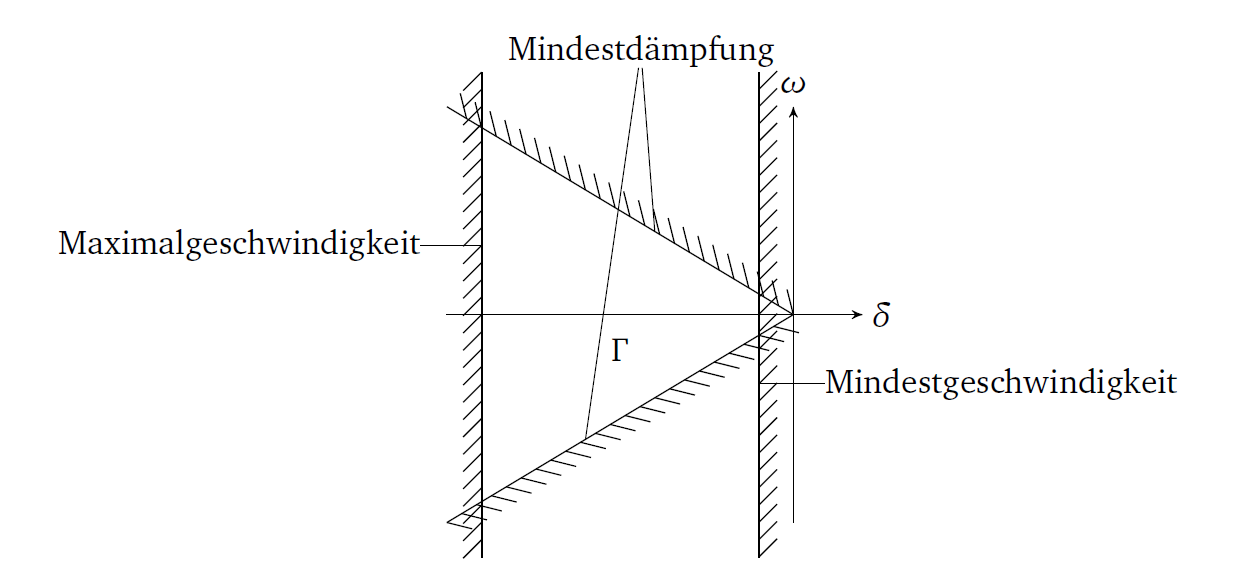
\includegraphics[width=\textwidth]{./Bilder/BedPolgebGrenzen.png}
	\caption{Bedeutung der Polgebietsgrenzen.\cite{RobReg}}
	\label{fig:BedPolgebGrenzen}
\end{figure}
Die Achsen beschreiben mit $\delta$ und $\omega$ den Real- bzw. Imaginärteil eines Poles $\lambda = \delta +\textnormal{j}\omega$.
Ziel ist nun einen Regler $\M{R}$ zu finden, welcher mit einer konstanten Zustandsrückführung alle Eigenwerte der verschiedenen Systeme in den vorher definierten Bereich $\Gamma$ platziert.
Über die Gebietsgrenzen von $\Gamma$ werden Anforderungen an Regel- bzw. Systemdynamiken entsprechend obiger Grafik \ref{fig:BedPolgebGrenzen} vorgegeben.
%, wie z.B. Schnelligkeit oder Schwingverhalten, vorgegeben werden.
Dabei kann es auch sinnvoll sein, unterschiedliche Polgebiete für die einzelnen Modelle zu definieren. Genauere Erklärungen zur mathematischen Beschreibung der Polgebietsgrenzen findet sich in entsprechender Literatur \cite{RobReg}.

Für das Verfahren ist es also nötig zu bewerten, wie gut die Fähigkeit eines bestimmten Reglers $\M{R}$ ist, die Eigenwerte des geregelten Systems im definierten Gebiet $\Gamma$ zu platzieren.
Hierfür soll eine Gütefunktion $J$ definiert werden. 
%Diese soll in Abhängigkeit von $\M{R}$ bewerten wie gut die Fähigkeit eines bestimmten Reglers ist die Eigenwerte des geregelten System im definierten Gebiet $\Gamma$ zu platzieren.
Seien die Eigenwerte des geregelten Systems gegeben durch 
$\lambda_{\rho i}(\M{R}) = \delta_{\rho i} (\M{R}) + \textnormal{j} \omega_{\rho i}(\M{R}) $ 
mit $\rho = 1,...,\Omega$ und $i = 1, ..., n$.
So soll gelten $\lambda_{\rho i}(\M{R}) \in \Gamma$. Liegen die Eigenwerte außerhalb des Bereichs, so soll $J(\M{R})$ große Werte annehmen.
Daraus lässt sich folgende Funktion 
\begin{equation}
	f\left(\delta_{\rho i}(\M{R}) ,\omega_{\rho i}(\M{R})\right) 
	\begin{cases}
		> 0 , \textnormal{wenn } \lambda_{\rho i}(\M{R}) \textnormal{ außerhalb von } \Gamma \textnormal{ liegt} \\
		= 0 , \textnormal{wenn } \lambda_{\rho i}(\M{R}) \textnormal{ auf dem Rand von } \Gamma \textnormal{ liegt} \\
		< 0 , \textnormal{wenn } \lambda_{\rho i}(\M{R}) \textnormal{ innerhalb von } \Gamma \textnormal{ liegt} \\
	\end{cases}
\end{equation}
ableiten.
Eine mögliche Gütefunktion ergibt sich dann zu 
\begin{equation}\label{eq:GueteMExp}
	J(\M{R}) = \sum_{\rho = 1}^{\Omega} \sum_{i=1}^{n} \mathrm{e}^{p_\rho f\left(\delta_{\rho i}(\M{R}) ,\omega_{\rho i}(\M{R})\right)}\,,
\end{equation}
wobei $p_\rho$ ein Gewichtungsfaktor darstellt.
Zur Lösung des Optimierungsproblems muss ein Regler $\M{R}^*$ gefunden werden, welcher die Gütefunktion $J(\M{R})$ minimiert.
\begin{equation}
	\M{R}^* = \textnormal{arg} \min_{\M{R}} J(\M{R})
\end{equation}
Für dieses nichtkonvexe Optimierungsproblem, ist ein numerisches Lösungsverfahren nötig.
Hier werden in der Regel Gradientenverfahren verwendet. Diese nutzen den Gradienten $\frac{\partial J(\M{R})}{\partial \M{R}}$ von $J$, um schrittweise das Minimum der Gütefunktion zu berechnen.\\
Der Gradient ergibt sich elementweise zu
\begin{equation}
	\frac{\partial J(\M{R})}{\partial r_{jh}} = \sum_{\rho = 1}^{\Omega} \sum_{i=1}^{n}
	p_\rho \mathrm{e}^{p_\rho f\left(\delta_{\rho i} ,\omega_{\rho i}\right)}
	\left(
	\frac{\partial f(\delta_{\rho i} ,\omega_{\rho i})}{\partial \delta_{\rho i}}
	\frac{\partial \delta_{\rho i} }{\partial r_{jh}} +
	\frac{\partial f(\delta_{\rho i} ,\omega_{\rho i})}{\partial \omega_{\rho i}}
	\frac{\partial \omega_{\rho i}}{\partial r_{jh}}
	\right)
\end{equation}
Hierbei gilt $j = 1,..,p$ und $h = 1,...,n$. Die Ableitungen $\frac{\partial f(\delta_{\rho i} ,\omega_{\rho i})}{\partial \delta_{\rho i}}$ sowie $	\frac{\partial f(\delta_{\rho i} ,\omega_{\rho i})}{\partial \omega_{\rho i}}$ ergeben sich aus den Grenzkurvenfunktionen des definierten Polgebiets $\Gamma$.
Zur Bestimmung von $\frac{\partial \delta_{\rho i} }{\partial r_{jh}} $ und $\frac{\partial \omega_{\rho i}}{\partial r_{jh}}$ nutzt man folgenden Zusammenhang
\begin{equation}
	\frac{\partial \lambda_{\rho i} }{\partial r_{jh}} = 	
	\frac{\partial \delta_{\rho i} }{\partial r_{jh}} +
	\textnormal{j}\frac{\partial \omega_{\rho i}}{\partial r_{jh}}
	\eqp
\end{equation}
Die Ableitungen ergeben sich dann zu 
\begin{equation}
		\frac{\partial \delta_{\rho i} }{\partial r_{jh}} = \Re\left\{ \frac{\partial \lambda_{\rho i} }{\partial r_{jh}}  \right\}
		\qquad \textnormal{und} \qquad
		\frac{\partial \omega_{\rho i}}{\partial r_{jh}} = \Im\left\{ \frac{\partial \lambda_{\rho i} }{\partial r_{jh}} \right\}
\end{equation}
Es gilt also $\frac{\partial \lambda_{\rho i} }{\partial r_{jh}}$ zu berechnen. Dies geschieht durch die beidseitige Ableitung des Rechtseigenwertproblems 
\begin{equation}
	\left( \M{A} - \M{B}\M{R} \right)\wt{v}{R i} = \lambda_{R i}\wt{v}{R i}
\end{equation}
nach einem Regelparameter $r_{jh}$. Bei vollständiger Zustandsrückführung ergibt sich die Ableitung dann zu
\begin{equation}\label{eq:AblLambdaR}
	\frac{\partial \lambda_{\rho i} }{\partial r_{jh}} = 
	- \frac{\w{w}^{\textnormal{T}}_{R i} \M{B} \wt{e}{j} \w{e}^{\textnormal{T}}_k \wt{v}{R i} }
		   {\w{w}^{\textnormal{T}}_{R i}  \wt{v}{R i}}
	\eqp
\end{equation}
Hier handelt es sich bei $\wt{w}{R i}$ um den $i-$ten Linkseigenvektor und bei $ \wt{v}{R i}$ um den entsprechenden Rechtseigenvektor. Die Vektoren $\wt{e}{j}$ und $\wt{e}{k}$ bezeichnen Einheitsvektoren in die $j-$te bzw. $k-$te Koordinatenrichtung.

Mit den Gleichungen (\ref{eq:GueteMExp}) und (\ref{eq:AblLambdaR}) kann nun ein optimaler Regler entworfen werden. Insgesamt können durch diese Methode alle $p\cdot n$ Koeffizienten in $\M{R}$ berechnet werden. Es ist jedoch auch möglich das Verfahren in Kombination mit strukturbeschränkten Reglern zu verwenden. Hierfür muss lediglich die Anzahl an Optimierungsvariablen  reduziert werden. Damit verändert man nicht mehr alle Reglerkoeffizienten in der Optimierung und es ist möglich, bestimmte Parameter fest oder von anderen abhängig zu wählen.

Nach dem Reglerentwurf ist eine Überprüfung der exakten Lage der Pole nötig. Dies soll sicherzustellen, dass alle Pole wie in Abbildung \ref{fig:PolgebKorrekt} dargestellt innerhalb des gewünschten Gebiets $\Gamma$ liegen. Tritt der in Abbildung \ref{fig:PolgebFalsch} beschriebene Fall auf, so muss der Reglerentwurf optimiert werden bis man zufriedenstellende Ergebnisse erzielt. In der Regel geschieht dies durch Änderung der Startwerte oder Gewichtungsfaktoren oder Polbereichsanpassungen.

\begin{figure}[h]
	\centering
	\begin{subfigure}[b]{0.35\textwidth}
		\centering
		\includegraphics[width=\textwidth]{./Bilder/PolgebKorrekt.png}
		\caption{Alle Pole der geregelten Strecke liegen innerhalb von $\Gamma$}
		\label{fig:PolgebKorrekt}
	\end{subfigure}
	\hspace{0.1\textwidth}
	\begin{subfigure}[b]{0.35\textwidth}
		\centering
		\includegraphics[width=0.85\textwidth]{./Bilder/PolgebFalsch.png}
		\caption{Einige Pole der geregelten Strecke liegen außerhalb von $\Gamma$}
		\label{fig:PolgebFalsch}
	\end{subfigure}
	\caption{Polgebiete mit Regelungseigenwerten \cite{Schaub}.}
	\label{fig:PolGeb}
\end{figure}
Nachdem das Konzept der Polbereichsplatzierung beschrieben wurde, soll im nächsten Abschnitt das Vorgehen bei der robusten Verkopplungsregelung auf Basis von Invarianzbetrachtungen erklärt werden.\\
